% -------------------------------- SVILUPPO -------------------------------------

\chapter{Probabilità}
\section{Spazi di probabilità}
\subsection{Probabilità uniforme}
\begin{itemize}
	\item P(A) = $\dfrac{|A|}{|\Omega|}$ = $\dfrac{Casi \ possibili}{Casi\  totali}$
\end{itemize}
\subsection{Probabilità condizionale}
\begin{itemize}
	\item $P(A \cap B) = P(A|B) \cdot P(B)$ (dipendenza)
	\item $P(A \cap B) = P(A) \cdot P(B)$  (indipendenza)
	\item $P(B|A) = \dfrac{P(A|B) \cdot P(B)}{P(A)}$
	\item $P(A|B) = P(A) = \dfrac{P(A \cap B)}{P(B)}$ (valido se c'è indipendenza)
\end{itemize}
\subsection{Formula di bayes}
\begin{itemize}
	\item $P(B|A) = \dfrac{P(A|B) \cdot P(B)}{P(A)}$
\end{itemize}
\subsection{Probabilità totali}
\begin{figure}[H]
	\centering{}
	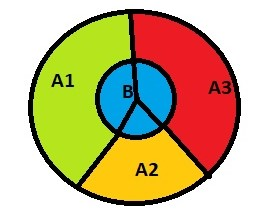
\includegraphics[width=\textwidth]{img/probtotali}
	\label{img:probtotali}
\end{figure}
	$P(B) = P(B \cap A_1) + P(B \cap A_2) + P(B \cap A_3)$ \\ \\
	= $P(A_1) \cdot P(B|A_1) + P(A_2) \cdot P(B|A_2) + P(A_3) \cdot P(B|A_3)$
\newpage
\section{Variabili aleatorie discrete}
\subsection{Densità discreta astratta}
Una funzione $p : \mathbb{R} \rightarrow \mathbb{R}$ \\
è una densità discreta astratta se e solo se: \\
\begin{itemize}
	\item $p(h) \neq 0$;
	\item $p(h) \geqslant 0 \ \ \forall \ \ h \in \mathbb{R}$;
	\item $\displaystyle \sum_{h \in \mathbb{R}} p(h) $ = 1;
\end{itemize}

\subsection{Distribuzioni discrete}
\textbf{Densità uniforme ($d_{x}(k)$)} \\ \\
$
\begin{cases}
	\dfrac{1}{n}\qquad  k = 1 \\  
	0\qquad			 altrimenti \\
\end{cases}
$	\\ \\ \\
\textbf{Densità di Bernoulli( $p_{x}(k)$ )} \\ \\
$
\begin{cases}
	P(A)\qquad\quad  	k = 1 \\  
	1 - P(A)\quad	k = 0 \\
	0\qquad\qquad\quad		altrimenti
\end{cases} \\
$ \\ 

\textbf{Densità binomiale ($p_{x}(k))$} \\ \\
$
\begin{cases}
	p^{k} \cdot(1-p)^{n - k} \cdot \binom{n}{k}\quad  k = 0,...,n \\  
	0\qquad\qquad\qquad\qquad\quad		 altrimenti \\
\end{cases}
$ \\ \\		

\textbf{Densità ipergeometrica (si considera a = successo)} \\ \\
$
\begin{cases}
	\dfrac{\binom{a}{k} \cdot \binom{b}{n - k}}{ \binom{a + b}{n}}\qquad  k = max(n - b), ..., min(n, b) \\  
	0\qquad\qquad\qquad			 altrimenti \\
\end{cases}
$ \\ \\	

\textbf{Densità geometrica modificata (cons. una sequenza con k - 1 insuccessi + 1 successo)} \\ \\
$
\begin{cases}
	(1 - p)^{k - 1} \cdot p\qquad  k = 1,2,3,... \\  
	0\qquad\qquad\qquad\quad			 altrimenti \\
\end{cases}
$ \\ \\	

\textbf{Densità geometrica standard (cons. una sequenza con k insuccessi prima di arrivare al successo)} \\ \\
$
\begin{cases}
	(1 - p)^{k} \cdot p\qquad  k = 1,2,3,... \\  
	0\qquad\qquad\qquad			 altrimenti \\
\end{cases}
$ \\ \\	

\textbf{Densità di Poisson} \\ \\
$
\begin{cases}
	e^{-\phi} \cdot \dfrac{\phi^{k}}{k!}\quad k = 1,2,3,.. \\
	0\qquad\quad\quad			 altrimenti \\
\end{cases}
$ \\ \\	

\newpage

\section{Variabili discrete multidimensionali}
\subsection{Funzione di ripartizione}
Sia $F_{x} : \mathbb{R} \rightarrow \mathbb{R}$, allora la sua funzione di ripartizione è la seguente :
\begin{itemize}
	\item $F_{x} = P(x \leq t)$
\end{itemize}

\subsection{Funzione di ripartizione del max}
Siano S, T due variabili aleatorie indipendenti e $Z = max(S, T)$, Allora: 
\begin{itemize}
	\item $F_{Z}(t) = F_{S}(t) \cdot F_{T}(t)$
\end{itemize}

\subsection{Funzione di ripartizione del min}
Siano S, T due variabili aleatorie indipendenti e W = min(S, T), Allora:
\begin{itemize}
	\item ($1 - F_{x}(k)) = (1 - F_{S}(t)) \cdot (1 - F_{T}(t))$
\end{itemize}

\newpage

\section{Valore atteso e varianza}
\subsection{Valore atteso}
\textbf{Definizione}
\begin{itemize}
	\item $E[x] = \displaystyle \sum_{h \in \mathbb{R}} d_{x}(h) \cdot h $; 
\end{itemize} 

\begin{flushleft}
	\textbf{Proprietà valore atteso}
\end{flushleft}
\begin{itemize}
	\item $E[x + y] = E[x] + E[y]$
	\item $E[x \cdot y] = E[x] \cdot E[y]$ (valido $\leftrightarrow$ x e y indipendenti)
\end{itemize}
\subsection{Varianza e covarianza}
\textbf{Definizione varianza} 
\begin{itemize}
	\item $Var(x) = E[(x - E[x])^2]$
\end{itemize}
\textbf{Definizione covarianza} 
\begin{itemize}
	\item $Cov(x, y) = E[x] \cdot E[y]$ 
\end{itemize}

\begin{flushleft}
	\textbf{Proprietà varianza}
\end{flushleft} 
\begin{itemize}
	\item $Var(x) = E[x^2] - E[x]^2$
	\item $Var(x + y) = var(x) + var(y)$
\end{itemize}
\textbf{Proprietà covarianza}
\begin{itemize}
	\item siano x, y indipendenti $\rightarrow Cov(x, y) = 0$
\end{itemize}

\newpage
\section{Variabili aleatorie continue}
\subsection{Densità continua}
x v.a continua, la sua densità è una funzione: \\ \\
$f_{x} : \mathbb{R} \rightarrow \mathbb{R}$ t.c : \\
\[ \int_{a}^{b} f_{x}(s) \,ds  = P(a \leq x \leq b)\]
\subsection{Densità e funzione di ripartizione astratta}
\textbf{Densità continua astratta}
\begin{itemize} 
	\item $f(s) \geq 0$
	\item  $ \int_{-\infty}^{\infty} f(s)ds  = 1 $
\end{itemize}
\textbf{Funzione di ripartizione astratta} \\ \\
$F : \mathbb{R} \rightarrow \mathbb{R}$ t.c : 
\begin{itemize}
	\item $\lim_{-\infty} F(t) = 0$ e $\lim_{+\infty}  F(t) = 1$
	\item F debolmente crescente
\end{itemize}
\subsection{Valore atteso}
\[ E[x] = \int_{-\infty}^{\infty} f_{x}(s) \,s \ ds\]
\textbf{Proprietà} \\
\begin{itemize}
	\item $E[ax + bx] = aE[x] + bE[y]$
	\item $E[x \cdot y] = E[x] \cdot E[y]$
	\item $E[\phi(x)] = \int_{-\infty}^{\infty} \phi(s)f_{x}(s)$ (se $\phi$:$\mathbb{R}$ $\rightarrow$ $\mathbb{R}$)
\end{itemize}
\newpage
\subsection{Varianza}
$Var(x) = E[x^2] - E[x]^2$ \\ \\
\textbf{Proprietà}
\begin{itemize}
	\item $Var(aX) = a^2 \cdot Var(X)$
	\item $Var(x + y) = Var(x) + Var(y)$
\end{itemize}
\subsection{Variabili uniformi continue}
$X \texttildelow U([a, b])$ 
\begin{itemize}
	\item $F_{x}(s) = \dfrac{s - a}{b - a}$ 
	\item $f_{x}(s) = \dfrac{1}{b - a}$	
	\item $E[x] = \dfrac{a + b}{2}$
	\item $Var(x) = \dfrac{(b - a)^2}{12}$
\end{itemize}
\subsection{Variabili esponenziali}
$X \texttildelow Exp(a)$
\begin{itemize}
	\item $F_{x}(s) = 1 - e^{as}$ 
	\item $f_{x}(s) = a \cdot e^{-as}$	
	\item $E[x] = \dfrac{1}{a}$
	\item $Var(x) = \dfrac{1}{a^2}$
\end{itemize}
\newpage
\subsection{Variabili normali(gaussiane)}
Standard : $\zeta_0 \texttildelow N(0,1)$ \\ \\
Generiche : $\zeta \texttildelow N(\mu,\sigma^2)$ \\ \\
\textbf{Proprietà}
\begin{itemize}
	\item $\zeta = \mu + \sigma \cdot \zeta_0$
	\item $F_{\zeta_0}(s) = \phi(s)$ (utilizziamo la tabella normale standard)
	\item $\phi(-s) = 1 - \phi(s)$
\end{itemize}
